\documentclass[12pt,a4paper]{article}
\usepackage{ctex}
\usepackage{amsmath,amscd,amsbsy,amssymb,latexsym,url,bm,amsthm}
\usepackage{epsfig,graphicx,subfigure}
\usepackage{enumitem,balance}
\usepackage{wrapfig}
\usepackage{mathrsfs,euscript}
\usepackage[usenames]{xcolor}
\usepackage{hyperref}
\usepackage[vlined,ruled,linesnumbered]{algorithm2e}
\hypersetup{colorlinks=true,linkcolor=black}
\usepackage[dvipsnames]{xcolor}
\usepackage{subcaption}
\usepackage[options]{algorithm2e}
\usepackage{algorithm}
\usepackage{algorithmic}
\usepackage{nameref}

\newtheorem{theorem}{Theorem}
\newtheorem{lemma}[theorem]{Lemma}
\newtheorem{proposition}[theorem]{Proposition}
\newtheorem{corollary}[theorem]{Corollary}
\newtheorem{exercise}{Exercise}
\newtheorem*{solution}{Solution}
\newtheorem{definition}{Definition}
\theoremstyle{definition}

\renewcommand{\thefootnote}{\fnsymbol{footnote}}

\newcommand{\postscript}[2]
 {\setlength{\epsfxsize}{#2\hsize}
  \centerline{\epsfbox{#1}}}

\renewcommand{\baselinestretch}{1.0}

\setlength{\oddsidemargin}{-0.365in}
\setlength{\evensidemargin}{-0.365in}
\setlength{\topmargin}{-0.3in}
\setlength{\headheight}{0in}
\setlength{\headsep}{0in}
\setlength{\textheight}{10.1in}
\setlength{\textwidth}{7in}
\makeatletter \renewenvironment{proof}[1][Proof] {\par\pushQED{\qed}\normalfont\topsep6\p@\@plus6\p@\relax\trivlist\item[\hskip\labelsep\bfseries#1\@addpunct{.}]\ignorespaces}{\popQED\endtrivlist\@endpefalse} \makeatother
\makeatletter
\renewenvironment{solution}[1][Solution] {\par\pushQED{\qed}\normalfont\topsep6\p@\@plus6\p@\relax\trivlist\item[\hskip\labelsep\bfseries#1\@addpunct{.}]\ignorespaces}{\popQED\endtrivlist\@endpefalse} \makeatother

\begin{document}
\noindent

%========================================================================
\noindent\framebox[\linewidth]{\shortstack[c]{
\Large{\textbf{Lab01-AlgorithmAnalysis}}\vspace{1mm}\\
CS2312-Algorithm and complexity, Xiaofeng Gao, Spring 2026.}}
\begin{center}
\footnotesize{\color{red}$*$ Contact TA Steven Chen for any questions. Include both your .pdf and .tex files in the uploaded .rar or .zip file.}

% Please write down your name, student id and email.
\footnotesize{\color{blue}$*$ Name:Hengtao Wu  \quad Student ID:524031910038 \quad Email: Eternity\_w@sjtu.edu.cn}
\end{center}


\begin{enumerate}
    % -------------------------------
    % Question 1
    % -------------------------------
    \item {\color{purple}(Minimal Counterexample Principle)}
    Prove that if one is given an unlimited supply of 6 cents, 10 cents, and 15 cents, one can make any amount of change larger than 29 cents.
    \begin{proof}
        Assume for contradiction that there exists an integer $n > 29$ that cannot be expressed in the form
        \[
        n = 6i + 10j + 15k,
        \]
        for nonnegative integers $i,j,k$. Let $n$ be the smallest such integer.
        
        First, observe that the following values can all be expressed:
        \[
        30 = 6\cdot5,\quad
        31 = 6 + 10 + 15,\quad
        32 = 6\cdot2 + 10\cdot2,\quad
        33 = 6\cdot3 + 15,\quad
        34 = 6\cdot4 + 10,\quad
        35 = 10\cdot2 + 15.
        \]
        Hence, every integer from 30 to 35 is representable, so the smallest counterexample must satisfy $n \ge 36$.Therefore, $n - 6 \ge 30 > 29$. By the minimality of $n$, the integer $n - 6$ is not a counterexample and can be written as
        \[
        n - 6 = 6i + 10j + 15k,
        \]
        for some nonnegative integers $i,j,k$.
        
        Then
        \[
        n = 6(i+1) + 10j + 15k,
        \]
        which shows that $n$ is also representable. This contradicts the assumption.
        
        Therefore, no such counterexample exists, and every integer $n > 29$ can be written as a combination of 6, 10, and 15.
    \end{proof}
        
    
    \smallskip
    % -------------------------------
    % Question 2
    % -------------------------------
    \item {\color{purple}{(Complexity Class)}}  
    Given the following functions:
    
    \[
    \quad f_1(n) = \lg n, \quad f_2(n) = 2^n, \quad f_3(n) = 1, \quad f_4(n) = \log^2{n}
    \]
    
    \[
    \quad f_5(n) = n, \quad f_6(n) = n!, \quad f_7(n) = n^n, \quad f_8(n) = 2^{\sqrt{\log n}}
    \]


    \begin{enumerate}
        \item Assume $\log n = \log_2 n \text{ and } \lg n = \log_{10} n$. Rank the functions $f(n)$ by growth rate, with "$\succ$" and "$\equiv$". e.g. $n^2\succ n \equiv 4n$. 
    \end{enumerate}
    \begin{solution}
        \[
        f_7(n)\succ f_6(n) \succ f_2(n) \succ f_5(n) \succ f_8(n) \succ f_4(n) \succ f_1(n) \succ f_3(n)
        \]
        \textbf{Brief Justification:}
    \begin{itemize}
        \item $f_3(n) = 1$: Constant time, the slowest.
        \item $f_1(n) = \lg n$: Logarithmic time, $\lg n = \Theta(\log n)$.
        \item $f_4(n) = \log^2 n$: Power of logarithm dominates standard logarithm.
        \item $f_8(n) = 2^{\sqrt{\log n}}$: Let $k = \log n$. We compare $k^2$ and $2^{\sqrt{k}}$. Exponential of $\sqrt{k}$ grows faster than polynomial of $k$, so $2^{\sqrt{\log n}} \succ \log^2 n$.
        \item $f_5(n) = n = 2^{\log n}$: Since $\log n \succ \sqrt{\log n}$, $2^{\log n} \succ 2^{\sqrt{\log n}}$. Thus $n \succ 2^{\sqrt{\log n}}$.
        \item $f_2(n) = 2^n$: Exponential function strictly dominates any polynomial function.
        \item $f_6(n) = n!$: $n! \sim \sqrt{2\pi n}(n/e)^n$, which grows strictly faster than $2^n$.
        \item $f_7(n) = n^n$: $n^n = n \cdot n \cdots n > n \cdot (n-1) \cdots 1 = n!$.
    \end{itemize}
    \end{solution}
    \smallskip
    % -------------------------------
    % Question 3
    % -------------------------------
    \item {\color{purple}(Time Complexity of Attention)}
    
    Attention is a fundamental component of the Transformer architecture. 
    The standard \textit{scaled dot-product attention} is defined as
    
    \begin{equation}
        \text{Attention}(Q, K, V) = 
        \text{softmax}\!\left(\frac{QK^{T}}{\sqrt{d_k}}\right)V
    \end{equation}
    
    where $Q$, $K$, and $V$ denote the \textit{query}, \textit{key}, and \textit{value} matrices, with $d_k$ representing the dimensionality of both $Q$ and $K$, and $d_v$ representing the dimensionality of $V$.
    
    Since the representational capacity of a single attention head is limited, modern Transformer models employ \textit{Multi-Head Attention}. This mechanism applies multiple attention operations in parallel and concatenates their outputs:
    
    \begin{equation}
        \text{MultiHead}(Q, K, V) =
        \text{Concat}(\text{head}_1, \dots, \text{head}_h) W^O
    \end{equation}
    
    where each attention head is defined as
    
    \begin{equation}
        \text{head}_i = 
        \text{Attention}(QW_i^Q, KW_i^K, VW_i^V),
    \end{equation}
    
    and $W_i^Q, W_i^K, W_i^V$ are learned parameters for the $i$-th head, while $W^O$ is the learned output projection matrix applied to the concatenated multi-head outputs. These $W$ matrices are not fixed inputs.
    
    Assume the following for the input sequence \(X \in \mathbb{R}^{n \times d_m}\):
    \begin{itemize}
        \item The input sequence length is $n$.
        \item The model dimension is $d_{m}$.
        \item The number of attention heads is $h$.
        \item Each head has dimensionality $d = d_{m}/h$.
        \item The \textit{query} and \textit{key} dimensionalities are equal: $d_k = d_v = d$.
    \end{itemize}
        
    \begin{enumerate}
        \item Write the pseudo-code for the \textbf{Multi-Head Attention} and \textbf{Scaled Dot-Product Attention} functions. Assume the input sequence $X$ has already been linearly projected into $Q$, $K$, and $V$. Clearly specify the input and output variable domains (i.e., dimensions) in your algorithm. For \textbf{Multi-Head Attention}, you can use $Attention()$ as a black box function that computes scaled dot-product attention.

        \item Analyze the \textbf{time complexity} of Scaled Dot-Product Attention in terms of $n$ and $d$. 
        
        {\color{blue}{(Detailed explanation required)}}

        {\color{red}{(HINT: $d_k = d_v = d$)}}
    
        \item Analyze the \textbf{time complexity} of Multi-Head Attention in terms of $n$ and $d_{m}$. 
        
        {\color{blue}{(Detailed explanation required)}}
        
        {\color{red}{(HINT: In practice, $n \gg d_{m}$. Consider relationship between $d$ and $d_{m}$)}}
    
    \end{enumerate}

    \begin{solution}
        \begin{enumerate}
        \item 
    The pseudo-code for \textbf{Scaled Dot-Product Attention} and \textbf{Multi-Head Attention} is presented below.
    
    \begin{algorithm}[H]
    \setcounter{AlgoLine}{0}
    \SetKwInOut{Input}{Input}\SetKwInOut{Output}{Output}
    \SetKwFunction{Softmax}{softmax}
    \Input{Query $Q \in \mathbb{R}^{n \times d}$, Key $K \in \mathbb{R}^{n \times d}$, Value $V \in \mathbb{R}^{n \times d}$}
    \Output{Context matrix $O \in \mathbb{R}^{n \times d}$}
    \BlankLine
    $Scores \leftarrow \frac{QK^T}{\sqrt{d}}$\tcp*[r]{Matrix mult: $(n \times d) \times (d \times n) \rightarrow n \times n$}\;
    $Weights \leftarrow \Softmax{$Scores$, \text{axis}=-1}$\tcp*[r]{Domain: $n \times n$}\;
    $O \leftarrow Weights \cdot V$\tcp*[r]{Matrix mult: $(n \times n) \times (n \times d) \rightarrow n \times d$}\;
    \Return $O$\;
    \caption{Scaled Dot-Product Attention}\label{algo_sdpa}
    \end{algorithm}
    
    \vspace{1em}
    
    \begin{algorithm}[H]
    \setcounter{AlgoLine}{0}
    \SetKwInOut{Input}{Input}\SetKwInOut{Output}{Output}
    \SetKwFunction{Attention}{Attention}\SetKwFunction{Concat}{Concat}
    \Input{Sequence $X \in \mathbb{R}^{n \times d_m}$, heads $h$, $d = d_m/h$\\
           Weight matrices $W_i^Q, W_i^K, W_i^V \in \mathbb{R}^{d_m \times d}$ for $i \in \{1, \dots, h\}$\\
           Output weight matrix $W^O \in \mathbb{R}^{d_m \times d_m}$}
    \Output{Final representation $Final\_Output \in \mathbb{R}^{n \times d_m}$}
    \BlankLine
    \For{$i\leftarrow 1$ \KwTo $h$}{
        $Q_i \leftarrow X W_i^Q$\tcp*[r]{Matrix mult: $(n \times d_m)\times(d_m\times d)\rightarrow n\times d$}\;
        $K_i \leftarrow X W_i^K$\tcp*[r]{Matrix mult: $(n \times d_m)\times(d_m\times d)\rightarrow n\times d$}\;
        $V_i \leftarrow X W_i^V$\tcp*[r]{Matrix mult: $(n \times d_m)\times(d_m\times d)\rightarrow n\times d$}\;
        $head_i \leftarrow \Attention{$Q_i, K_i, V_i$}$\tcp*[r]{Domain: $n \times d$}\;
    }
    $ConcatOutput \leftarrow \Concat{$head_1, \dots, head_h$}$\tcp*[r]{Domain: $n \times (h \cdot d) \equiv n \times d_m$}\;
    $FinalOutput \leftarrow ConcatOutput \cdot W^O$\tcp*[r]{Matrix mult: $(n \times d_m) \times (d_m \times d_m) \rightarrow n \times d_m$}\;
    \Return $FinalOutput$\;
    \caption{Multi-Head Attention}\label{algo_mha}
    \end{algorithm}
        \item \label{ques_b} The time complexity of \textbf{Scaled Dot-Product Attention} is $\mathcal{O}(n^2 d)$.
        The computation consists of three main steps:
        \begin{itemize}
            \item \textbf{Step 1 ($QK^T$):} Multiplying the query matrix $Q \in \mathbb{R}^{n \times d}$ and the transposed key matrix $K^T \in \mathbb{R}^{d \times n}$ takes $\mathcal{O}(n\cdot d\cdot n) = \mathcal{O}(n^2 d)$. The scaling by $\sqrt{d}$ takes $\mathcal{O}(n^2)$.
            \item \textbf{Step 2 ($\text{softmax}$):} Applying the softmax function to the $n \times n$ score matrix takes $\mathcal{O}(n^2)$.
            \item \textbf{Step 3 ($\text{Weights} \cdot V$):} Multiplying the $n\times n$ weight matrix with the value matrix $V \in \mathbb{R}^{n \times d}$ takes $\mathcal{O}(n \cdot n \cdot d) = \mathcal{O}(n^2 d)$.
        \end{itemize}
        Summing these up, the dominant term is clearly the matrix multiplication, yielding a total time complexity of $\mathcal{O}(n^2 d)$.

        \item The time complexity of \textbf{Multi-Head Attention} is $\mathcal{O}(n^2 d_m)$. The computation consists of four main steps:
        \begin{itemize}
            \item \textbf{Step 1 ($X W_i$):} During the loop, multiplying the input matrix $X \in \mathbb{R}^{n \times d_m}$ with the projection matrices $W_i^{Q/K/V}$ takes $\mathcal{O}(n\cdot d_m\cdot d)$. Since the loop runs $h$ times and $h\cdot d = d_m$, this step takes a total of $\mathcal{O}(n\cdot d_m^2)$.
            \item \label{c_step2} \textbf{Step 2 (Attention):} From Question \ref{ques_b}, we know that the \textit{Attention} operation in each iteration takes $\mathcal{O}(n^2 d)$.Hence, loop for all $h$ heads takes $\mathcal{O}(n^2\cdot d\cdot h) = \mathcal{O}(n^2 d_m)$.
            \item \textbf{Step 3 (Concat):} Because this step only needs to concatenate the $h$ matrices, it takes $\mathcal{O}(n\cdot d\cdot h) = \mathcal{O}(n d_m)$.
            \item \textbf{Step 4 (Final):} Similar to the matrix multiplications discussed above, multiplying the concatenated matrix with the output matrix takes $\mathcal{O}(n\cdot d_m \cdot d_m) = \mathcal{O}(n d_m^2)$.
        \end{itemize}
        In summary, since $n \gg d_m$ in practice, the term $\mathcal{O}(n^2 d_m)$ grows much faster than $\mathcal{O}(n d_m^2)$. This indicates that \hyperref[c_step2]{Step 2} is the dominant, bringing the overall time complexity of Multi-Head Attention to $\mathcal{O}(n^2 d_m)$.
                
        \end{enumerate}
    \end{solution}
    \smallskip
    % -------------------------------
    % Question 4
    % -------------------------------
    \item {\color{purple}(Divide-and-Conquer Analysis)}
    A tromino is an $L$-shaped tile formed by three connected $1 \times 1$ squares. Given an $n \times n$ (where $n = 2^k$, $k \geq 1$) board with a missing square cell, your task is to fill the remaining cells with trominoes. Trominoes can be oriented in any arbitrary way, but they should cover all the cells of the board except the missing one exactly and with no overlaps.

    \begin{figure}[h]
        \hspace{0.15\textwidth}
        \begin{minipage}{0.4\textwidth}
            \subfigure[Tromino]
            {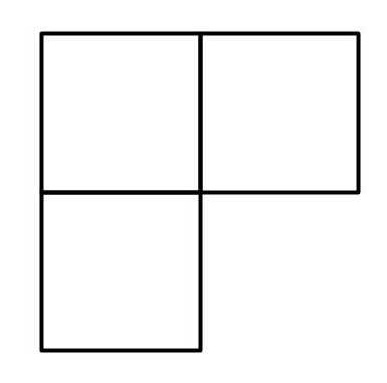
\includegraphics[scale=1]{Fig-Tromino Example.jpg}}
        \end{minipage}
        \begin{minipage}{0.4\textwidth}
            \subfigure[Board]
            {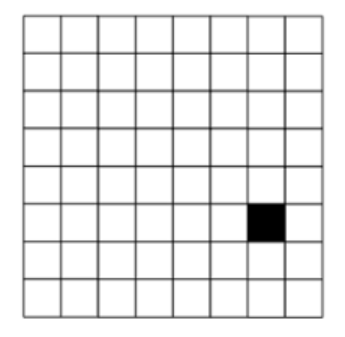
\includegraphics[scale=1]{Fig-Tiling Problem.png}}
        \end{minipage}
    \end{figure}
    
    \begin{enumerate}
        \item Design a divide-and-conquer method for the tromino tiling problem. Explain your algorithm. Do not provide pseudo-code.

        {\color{red}{(HINT: Place the first tromino at the center of board)}}

        \item Express the cost of solving the problem as a recurrence relation and use the Master Theorem to find the running time.
    \end{enumerate}
    \begin{solution}
        \begin{enumerate}
            \item \textbf{Divide-and-Conquer Algorithm:}
            \begin{itemize}
                \item \textbf{Base Case:} First, we establish the base case. When $k = 1$ (i.e., $n = 2$), the board has exactly one missing cell, and the remaining three cells naturally form an L-shape.
                \item \textbf{Divide and Place:} For a general $n \times n$ board, we logically divide it into four $(n/2) \times (n/2)$ quadrants. We place the first tromino at the exact center of the board. We then adjust its orientation so that its three squares fall into the three quadrants that do \textit{not} contain the originally missing cell. 
                \item \textbf{Conquer (Recursive Step):} If we treat the originally missing cell and the three cells covered by the center tromino all as "occupied" cells, we can observe that each of the four quadrants now has exactly one occupied cell and a size of $n' = n/2$. We can then recursively apply this exact algorithm to fill the remaining cells in each of the four quadrants until we reach the base case.
            \end{itemize}
            \item Since the problem is divided into four subproblems at each step, with the problem size reduced to $n/2$, and each merge operation involves placing only a single tromino (i.e., constant time $\mathcal{O}(1)$), we can formulate the following recurrence relation:
                \[
                    T(n) = 4T\left(\frac{n}{2}\right) + \mathcal{O}(1).
                \]
            According to the Master Theorem, where $f(n) = \mathcal{O}(n^d)$ with $d = 0$, we have $d = 0 < \log_b a = \log_2 4 = 2$. Therefore, we get $T(n) = \mathcal{O}(n^{\log_b a}) = \mathcal{O}(n^2)$.
        \end{enumerate}
    \end{solution}


    
\end{enumerate}






%========================================================================
\end{document}
